% ============================================================
% Cours : Équations Différentielles Linéaires du Premier Ordre
% Pôle Formation UIMM - CVDL
% BTS Industriel - Mathématiques
% Auteur : S. JAUBERT
% ============================================================
\documentclass[a4paper,11pt]{article}

% ----- Encodage et langue -----
\usepackage[utf8]{inputenc}
\usepackage[T1]{fontenc}
\usepackage[french]{babel}

% ----- Polices sans-serif -----
\usepackage{helvet}
\renewcommand{\familydefault}{\sfdefault}

% ----- Mise en page -----
\usepackage[top=3cm, bottom=2.5cm, left=2cm, right=2cm, headheight=2cm]{geometry}

% ----- Mathématiques -----
\usepackage{amsmath,amssymb,amsfonts}

% ----- Graphiques et couleurs -----
\usepackage{graphicx}
\usepackage[dvipsnames,table]{xcolor}
\usepackage{tikz}
\usetikzlibrary{arrows.meta, decorations.pathmorphing, calc}
\usepackage{pgfplots}
\pgfplotsset{compat=1.18}

% ----- Boîtes colorées -----
\usepackage[most]{tcolorbox}

% ----- Code / algorithmes -----
\usepackage{listings}

% ----- En-tête et pied de page -----
\usepackage{fancyhdr}

% ----- Hyperliens -----
\usepackage{hyperref}
\hypersetup{colorlinks=true, linkcolor=uimmblue, urlcolor=uimmblue}

% ----- Enumération personnalisée -----
\usepackage{enumitem}

% ----- Tableaux -----
\usepackage{booktabs,array}

% ============================================================
% CHARTE GRAPHIQUE UIMM
% ============================================================
\definecolor{uimmblue}{HTML}{005C85}
\definecolor{uimmred}{HTML}{D31326}
\definecolor{uimmlightblue}{HTML}{E8F1F8}
\definecolor{uimmgray}{HTML}{333333}
\definecolor{uimmlightgray}{HTML}{F5F5F5}

% ----- Styles des sections -----
\usepackage{titlesec}
\titleformat{\section}
  {\LARGE\bfseries\color{uimmblue}}
  {\thesection.}{0.5em}{}[\vspace{2pt}{\color{uimmblue}\titlerule[1.5pt]}]
\titleformat{\subsection}
  {\Large\bfseries\color{uimmblue}}
  {\thesubsection.}{0.5em}{}
\titleformat{\subsubsection}
  {\large\bfseries\color{uimmblue!80!black}}
  {\thesubsubsection.}{0.5em}{}

% ----- Puces personnalisées -----
\setlist[itemize,1]{label={\color{uimmblue}\textbullet}}
\setlist[itemize,2]{label={\color{uimmblue}--}}
\setlist[enumerate,1]{label={\color{uimmblue}\textbf{\arabic*.}}}

% ----- Style listings -----
\lstdefinestyle{uimmpython}{
  basicstyle=\ttfamily\small,
  keywordstyle=\color{uimmblue}\bfseries,
  commentstyle=\color{green!50!black}\itshape,
  stringstyle=\color{uimmred},
  numbers=left, numberstyle=\tiny\color{uimmgray}, numbersep=8pt,
  showstringspaces=false, breaklines=true, frame=single,
  rulecolor=\color{uimmblue}, backgroundcolor=\color{uimmlightgray},
  language=Python
}

% ============================================================
% BOÎTES TCOLORBOX
% ============================================================
\newtcolorbox{definition}[1][]{%
  colback=uimmlightblue, colframe=uimmblue,
  fonttitle=\bfseries\color{white}, title={\textsf{Définition}~#1},
  coltitle=white, boxrule=1pt, arc=3pt,
  left=8pt, right=8pt, top=6pt, bottom=6pt, before skip=10pt, after skip=10pt}

\newtcolorbox{theoreme}[1][]{%
  colback=uimmlightblue!50, colframe=uimmblue!80!black,
  fonttitle=\bfseries\color{white}, title={\textsf{Théorème / Propriété}~#1},
  coltitle=white, boxrule=1.2pt, arc=3pt,
  left=8pt, right=8pt, top=6pt, bottom=6pt, before skip=10pt, after skip=10pt}

\newtcolorbox{methode}[1][]{%
  colback=green!5, colframe=green!50!black,
  fonttitle=\bfseries\color{white}, title={\textsf{Méthode}~#1},
  coltitle=white, boxrule=1pt, arc=3pt,
  left=8pt, right=8pt, top=6pt, bottom=6pt, before skip=10pt, after skip=10pt}

\newtcolorbox{exemple}[1][]{%
  colback=orange!5, colframe=orange!70!black,
  fonttitle=\bfseries\color{white}, title={\textsf{Exemple}~#1},
  coltitle=white, boxrule=1pt, arc=3pt,
  left=8pt, right=8pt, top=6pt, bottom=6pt, before skip=10pt, after skip=10pt}

\newtcolorbox{remarque}[1][]{%
  colback=uimmlightgray, colframe=uimmgray,
  fonttitle=\bfseries, title={\textsf{Remarque}~#1},
  boxrule=0.8pt, arc=3pt,
  left=8pt, right=8pt, top=6pt, bottom=6pt, before skip=10pt, after skip=10pt}

\newtcolorbox{appliindus}[1][]{%
  colback=uimmred!5, colframe=uimmred!80!black,
  fonttitle=\bfseries\color{white}, title={\textsf{$\triangleright$ Application industrielle}~#1},
  coltitle=white, boxrule=1.2pt, arc=4pt,
  left=8pt, right=8pt, top=6pt, bottom=6pt, before skip=10pt, after skip=10pt}

% ============================================================
% EN-TÊTE / PIED DE PAGE
% ============================================================
\pagestyle{fancy}
\fancyhf{}
\renewcommand{\headrulewidth}{0pt}
\renewcommand{\footrulewidth}{0pt}

\fancyhead[L]{\raisebox{-0.5\height}{
\includegraphics[height=1.5cm]{logo_uimm_placeholder.jpg}}}
\fancyhead[C]{%
  \begin{minipage}{8cm}\centering
    {\small\color{uimmblue}\textbf{Pôle Formation UIMM - CVDL}}\\
    {\footnotesize\color{uimmgray} BTS Industriel -- Mathématiques}
  \end{minipage}}
\fancyhead[R]{{\small\color{uimmblue}\textbf{MOD06}}}
\fancyfoot[C]{%
  {\color{uimmblue}\rule{\textwidth}{1pt}}\\[2pt]
  {\footnotesize\color{uimmgray} Pôle Formation UIMM -- Centre-Val de Loire \hfill S. JAUBERT \hfill \thepage}}

% ============================================================
% PAGE DE TITRE
% ============================================================
\begin{document}

\begin{titlepage}
\begin{tikzpicture}[remember picture, overlay]
  \fill[uimmblue] (current page.north west) rectangle ([yshift=-4cm]current page.north east);
  \node[anchor=north west] at ([xshift=2cm, yshift=-0.5cm]current page.north west)
    {
\includegraphics[height=3cm]{logo_uimm_placeholder.jpg}};
  \node[anchor=north east, white, font=\large\bfseries] at ([xshift=-2cm, yshift=-1.5cm]current page.north east)
    {Pôle Formation UIMM - CVDL};
  \node[anchor=north east, white, font=\small, align=right] at ([xshift=-2cm, yshift=-2.2cm]current page.north east)
    {BTS Industriel -- Mathématiques\\[2pt]S. Jaubert};
  \fill[uimmred] ([yshift=-4cm]current page.north west) rectangle ([yshift=-4.4cm]current page.north east);
  \node[anchor=center, text width=14cm, align=center] at ([yshift=-1cm]current page.center) {
    {\fontsize{28}{34}\selectfont\bfseries\color{uimmblue} Équations Différentielles\\[6pt] Linéaires du Premier Ordre}\\[20pt]
    {\Large\color{uimmgray} Module 06 -- Analyse}\\[12pt]
    {\large\color{uimmgray}\textit{Applications industrielles et physiques}}
  };
  \fill[uimmblue] ([yshift=1.5cm]current page.south west) rectangle (current page.south east);
  \node[anchor=center, white, font=\small] at ([yshift=0.75cm]current page.south) {
    Pôle Formation UIMM -- Centre-Val de Loire $\bullet$ La Fabrique de l'Avenir};
\end{tikzpicture}
\end{titlepage}

% ============================================================
% FICHE MODULE
% ============================================================
\thispagestyle{fancy}
\vspace*{0.5cm}
\begin{center}
{\LARGE\bfseries\color{uimmblue} MOD06 -- Équations Différentielles}\\[6pt]
{\large\color{uimmgray} Support de cours}\\[4pt]
{\normalsize\color{uimmgray} Auteur : S. JAUBERT \hspace{1cm} Formation : BTS Industriel Groupement B}
\end{center}
\vspace{0.8cm}

\begin{tcolorbox}[colback=uimmlightblue!30, colframe=uimmblue,
  title={\textbf{\textsf{Fiche du Module}}}, fonttitle=\large\bfseries\color{white},
  coltitle=white, boxrule=1.2pt, arc=4pt, left=10pt, right=10pt, top=8pt, bottom=8pt]
\renewcommand{\arraystretch}{1.6}
\begin{tabular}{@{}>{\bfseries\color{uimmblue}}l @{\hspace{12pt}} p{12cm}@{}}
Bloc / Période : & Semestre 3 \\
Module :         & {[MOD06]} Équations Différentielles \\
Séquence :       & {[S01]} Premier ordre \\
Thème :          & Résolution des équations différentielles linéaires du premier ordre à coefficients constants -- Applications physiques et industrielles \\
\end{tabular}
\end{tcolorbox}
\vspace{0.5cm}

\begin{tcolorbox}[colback=white, colframe=uimmblue!80!black,
  title={\textbf{\textsf{Séquence et Compétences travaillées}}}, fonttitle=\large\bfseries\color{white},
  coltitle=white, boxrule=1pt, arc=4pt, left=10pt, right=10pt, top=8pt, bottom=8pt]

\textbf{\color{uimmblue} [S01] -- Premier ordre}
\begin{itemize}[leftmargin=1.5cm]
  \item[\textbf{\color{uimmblue}[C01]}] Résoudre une équation différentielle du premier ordre (à la main ou via logiciel)
  \item[\textbf{\color{uimmblue}[C02]}] Déterminer la solution vérifiant une condition initiale donnée
  \item[\textbf{\color{uimmblue}[C03]}] Représenter à l'aide d'un logiciel la famille des courbes solutions
\end{itemize}
\end{tcolorbox}
\vspace{0.4cm}

\begin{remarque}[-- Positionnement du cours]
Ce support traite la \textbf{Séquence S01 -- Premier ordre}. Il précède le cours sur le second ordre et fournit les bases du raisonnement : équation homogène, solution particulière, condition initiale, régime transitoire et régime permanent. Prérequis : dérivées et primitives, fonction exponentielle (MOD04). Les applications sont issues de l'électricité, de la thermique, de la mécanique et de la chimie.
\end{remarque}

\newpage
\tableofcontents
\newpage

% ============================================================
% SECTION 1 : INTRODUCTION
% ============================================================
\section{Introduction et motivations}

Une équation différentielle relie une fonction inconnue à ses dérivées. Elle traduit une \textbf{loi d'évolution} : la façon dont une grandeur varie dépend de sa valeur actuelle. C'est le langage naturel des phénomènes qui évoluent dans le temps.

\begin{remarque}
Les équations différentielles du premier ordre décrivent une multitude de situations industrielles :
\begin{itemize}
  \item l'\textbf{établissement d'un courant} dans une bobine (circuit RL) ;
  \item la \textbf{charge d'un condensateur} (circuit RC) ;
  \item le \textbf{refroidissement} d'une pièce après traitement thermique ;
  \item la \textbf{cinétique} d'une réaction chimique du premier ordre ;
  \item la \textbf{vitesse} d'un mobile soumis à un frottement visqueux.
\end{itemize}
Toutes obéissent au même modèle mathématique. Le maîtriser, c'est comprendre d'un coup tous ces phénomènes.
\end{remarque}

\subsection{Objectifs du cours}
À l'issue de ce cours, l'étudiant sera capable de :
\begin{enumerate}
  \item identifier une équation différentielle linéaire du premier ordre à coefficients constants ;
  \item résoudre l'équation homogène associée ;
  \item déterminer une solution particulière selon le second membre ;
  \item appliquer une condition initiale pour trouver la solution unique ;
  \item interpréter la solution (constante de temps, régime transitoire et régime permanent) ;
  \item mettre en {\oe}uvre la méthode d'Euler pour une résolution approchée.
\end{enumerate}

% ============================================================
% SECTION 2 : GÉNÉRALITÉS
% ============================================================
\newpage
\section{Généralités}

\subsection{Définition}

\begin{definition}
Une \textbf{équation différentielle linéaire du premier ordre à coefficients constants} est une équation de la forme :
\[
\boxed{a\,y'(t) + b\,y(t) = c(t)}
\]
où :
\begin{itemize}
  \item $a$ et $b$ sont des constantes réelles avec $a \neq 0$ ;
  \item $y(t)$ est la fonction inconnue et $y'(t)$ sa dérivée ;
  \item $c(t)$ est le \textbf{second membre} (fonction connue).
\end{itemize}
En divisant par $a$, on se ramène souvent à la \textbf{forme normalisée} :
\[
y'(t) + \alpha\,y(t) = f(t), \qquad \text{avec } \alpha = \frac{b}{a}.
\]
\end{definition}

\begin{definition}
Lorsque le second membre est nul, l'équation est dite \textbf{homogène} (ou \textbf{sans second membre}) :
\[
a\,y'(t) + b\,y(t) = 0.
\]
\end{definition}

\begin{exemple}[-- Vocabulaire]
\renewcommand{\arraystretch}{1.4}
\begin{center}
\begin{tabular}{>{\raggedright}p{6.5cm} c c}
\toprule
\textbf{Équation} & \textbf{Ordre} & \textbf{Type} \\
\midrule
$y' + 3y = 0$ & 1 & Homogène \\
$2y' + y = 10$ & 1 & Second membre constant \\
$y' - y = e^{2t}$ & 1 & Second membre exponentiel \\
$0{,}5\,y' + y = \cos(t)$ & 1 & Second membre sinusoïdal \\
\bottomrule
\end{tabular}
\end{center}
\end{exemple}

\subsection{Mise en équation de quelques phénomènes}

\begin{appliindus}[-- Circuit RL : établissement du courant]
Une bobine d'inductance $L$ et une résistance $R$ en série sont branchées sur une tension constante $E$. La loi des mailles donne :
\[
L\,\frac{di}{dt} + R\,i = E.
\]
\textbf{Identification :} $a = L$, $b = R$, $c(t) = E$ (constant).
\end{appliindus}

\begin{appliindus}[-- Circuit RC : charge d'un condensateur]
Une résistance $R$ et un condensateur $C$ en série sous une tension $E$ vérifient, pour la tension $u_C$ aux bornes du condensateur :
\[
RC\,\frac{du_C}{dt} + u_C = E.
\]
\textbf{Identification :} $a = RC$, $b = 1$, $c(t) = E$.
\end{appliindus}

\begin{appliindus}[-- Refroidissement (loi de Newton)]
La température $\theta(t)$ d'une pièce placée dans un milieu à température ambiante $\theta_a$ vérifie :
\[
\theta'(t) = -k\,\big(\theta(t) - \theta_a\big) \;\Longleftrightarrow\; \theta'(t) + k\,\theta(t) = k\,\theta_a,
\]
où $k > 0$ est le coefficient d'échange thermique.
\end{appliindus}

% ============================================================
% SECTION 3 : ÉQUATION HOMOGÈNE
% ============================================================
\newpage
\section{Résolution de l'équation homogène}

\begin{theoreme}[-- Solutions de l'équation homogène]
Les solutions de l'équation homogène $y'(t) + \alpha\,y(t) = 0$ sont les fonctions :
\[
\boxed{y(t) = C\,e^{-\alpha t}}
\]
où $C$ est une constante réelle quelconque. Il y a donc une \textbf{infinité} de solutions (une famille de courbes).
\end{theoreme}

\begin{remarque}
Attention au signe : l'équation $y' + \alpha y = 0$ donne $e^{-\alpha t}$. Pour la forme $a y' + b y = 0$, on a $\alpha = b/a$, donc $y(t) = C\,e^{-\frac{b}{a} t}$.
\end{remarque}

\begin{methode}[-- Résoudre une équation homogène]
\begin{enumerate}
  \item Mettre l'équation sous la forme $y' + \alpha y = 0$ (diviser par $a$) ;
  \item lire $\alpha$ ;
  \item écrire directement $y(t) = C\,e^{-\alpha t}$.
\end{enumerate}
\end{methode}

\begin{exemple}[-- Trois résolutions]
\begin{itemize}
  \item $y' + 3y = 0$ \; donne \; $y(t) = C\,e^{-3t}$ ;
  \item $2y' + y = 0 \iff y' + 0{,}5\,y = 0$ \; donne \; $y(t) = C\,e^{-0{,}5t}$ ;
  \item $5y' - 10y = 0 \iff y' - 2y = 0$ \; donne \; $y(t) = C\,e^{2t}$.
\end{itemize}
\end{exemple}

\begin{center}
\begin{tikzpicture}
\begin{axis}[
  width=12cm, height=6cm,
  xlabel={$t$}, ylabel={$y(t)$},
  xmin=0, xmax=4, ymin=0, ymax=5,
  axis lines=left, tick style={uimmgray}, every axis label/.style={uimmblue},
  samples=120, domain=0:4,
  legend style={draw=none, at={(0.98,0.98)}, anchor=north east, font=\small}
]
\addplot[uimmblue, very thick] {4*exp(-1.2*x)};   \addlegendentry{$C=4$}
\addplot[uimmred, very thick] {2.5*exp(-1.2*x)};  \addlegendentry{$C=2{,}5$}
\addplot[uimmgray, very thick] {1*exp(-1.2*x)};   \addlegendentry{$C=1$}
\end{axis}
\end{tikzpicture}\\
{\footnotesize\color{uimmgray} Famille des solutions de $y' + 1{,}2\,y = 0$ : chaque valeur de $C$ donne une courbe.}
\end{center}

% ============================================================
% SECTION 4 : SECOND MEMBRE
% ============================================================
\newpage
\section{Équation complète avec second membre}

\begin{theoreme}[-- Structure de la solution générale]
La solution générale de $a\,y' + b\,y = c(t)$ s'écrit :
\[
\boxed{y(t) = y_h(t) + y_p(t)}
\]
où :
\begin{itemize}
  \item $y_h(t) = C\,e^{-\alpha t}$ est la solution générale de l'équation homogène (\textbf{régime transitoire}, il s'éteint) ;
  \item $y_p(t)$ est \textbf{une} solution particulière de l'équation complète (\textbf{régime permanent}, ce qui reste).
\end{itemize}
\end{theoreme}

\subsection{Second membre constant}

\begin{methode}[-- $c(t) = K$ (constante), avec $b \neq 0$]
On cherche une solution particulière \textbf{constante} $y_p = \dfrac{K}{b}$ (obtenue en écrivant $y_p' = 0$ dans l'équation).
\end{methode}

\begin{exemple}
$y' + 2y = 6$.
\begin{itemize}
  \item Solution particulière : $y_p = \dfrac{6}{2} = 3$.
  \item Homogène : $y_h = C\,e^{-2t}$.
  \item \textbf{Solution générale :} $y(t) = C\,e^{-2t} + 3$.
\end{itemize}
\end{exemple}

\subsection{Second membre polynomial}

\begin{methode}[-- $c(t)$ polynôme de degré $n$]
On cherche $y_p$ sous forme d'un polynôme de même degré $n$, puis on identifie les coefficients.
\end{methode}

\begin{exemple}
$y' + y = 2t + 1$. On pose $y_p = \beta t + \gamma$, donc $y_p' = \beta$.
\[
\beta + \beta t + \gamma = 2t + 1 \;\Rightarrow\; \beta = 2 \text{ et } \beta + \gamma = 1 \Rightarrow \gamma = -1.
\]
Donc $y_p = 2t - 1$ et $y(t) = C\,e^{-t} + 2t - 1$.
\end{exemple}

\subsection{Second membre exponentiel}

\begin{methode}[-- $c(t) = P\,e^{\gamma t}$]
\begin{itemize}
  \item si $\gamma \neq -\alpha$ (le taux du second membre n'est pas celui de l'homogène) : $y_p = \lambda\,e^{\gamma t}$ ;
  \item si $\gamma = -\alpha$ (résonance) : $y_p = \lambda\,t\,e^{\gamma t}$.
\end{itemize}
On détermine $\lambda$ par substitution.
\end{methode}

\begin{exemple}
$y' - y = e^{2t}$. Ici $\alpha = -1$, et $\gamma = 2 \neq 1$. On pose $y_p = \lambda e^{2t}$ :
\[
2\lambda e^{2t} - \lambda e^{2t} = \lambda e^{2t} = e^{2t} \;\Rightarrow\; \lambda = 1.
\]
Donc $y_p = e^{2t}$ et $y(t) = C\,e^{t} + e^{2t}$.
\end{exemple}

\subsection{Second membre sinusoïdal}

\begin{methode}[-- $c(t) = P\cos(\omega t) + Q\sin(\omega t)$]
On cherche $y_p(t) = \lambda\cos(\omega t) + \mu\sin(\omega t)$, puis on identifie les coefficients de $\cos$ et $\sin$. C'est le \textbf{régime sinusoïdal forcé}, courant en électricité.
\end{methode}

\begin{remarque}[-- Méthode générale : variation de la constante]
Quand le second membre ne rentre dans aucun cas type, on peut toujours utiliser la \textbf{variation de la constante} : on cherche la solution sous la forme $y(t) = C(t)\,e^{-\alpha t}$, où $C$ devient une fonction. Cette méthode générale n'est pas exigible au BTS mais un logiciel de calcul formel la met en {\oe}uvre automatiquement.
\end{remarque}

% ============================================================
% SECTION 5 : CONDITION INITIALE
% ============================================================
\newpage
\section{Détermination de la constante par la condition initiale}

\begin{theoreme}[-- Problème de Cauchy]
L'équation $a\,y' + b\,y = c(t)$ admet une \textbf{unique} solution vérifiant une condition initiale donnée $y(t_0) = y_0$. Cette condition détermine la constante $C$.
\end{theoreme}

\begin{methode}[-- Résoudre un problème de Cauchy]
\begin{enumerate}
  \item écrire la solution générale $y(t) = C\,e^{-\alpha t} + y_p(t)$ ;
  \item remplacer $t$ par $t_0$ et écrire $y(t_0) = y_0$ ;
  \item résoudre l'équation obtenue pour trouver $C$ ;
  \item écrire la solution finale (unique).
\end{enumerate}
\end{methode}

\begin{exemple}[-- Résolution complète]
Résoudre $y' + 2y = 6$ avec $y(0) = 0$.
\begin{itemize}
  \item Solution générale (vue plus haut) : $y(t) = C\,e^{-2t} + 3$.
  \item Condition initiale : $y(0) = C + 3 = 0 \Rightarrow C = -3$.
  \item \textbf{Solution :} $y(t) = 3 - 3\,e^{-2t} = 3\big(1 - e^{-2t}\big)$.
\end{itemize}
La grandeur part de $0$ et tend vers $3$ : c'est la forme typique d'un établissement (charge, montée en régime).
\end{exemple}

% ============================================================
% SECTION 6 : CONSTANTE DE TEMPS
% ============================================================
\newpage
\section{Constante de temps, régime transitoire et régime permanent}

Pour une équation $y' + \alpha y = f$ à second membre constant, la solution est de la forme $y(t) = y_\infty + (y_0 - y_\infty)\,e^{-\alpha t}$. On pose la \textbf{constante de temps} $\tau = \dfrac{1}{\alpha}$.

\begin{definition}
La \textbf{constante de temps} $\tau$ caractérise la rapidité du phénomène :
\[
y(t) = y_\infty + (y_0 - y_\infty)\,e^{-t/\tau}.
\]
$y_\infty$ est la valeur du \textbf{régime permanent} (limite quand $t \to +\infty$) ; le terme en $e^{-t/\tau}$ est le \textbf{régime transitoire}, qui s'éteint.
\end{definition}

\begin{theoreme}[-- Repères à connaître]
\begin{itemize}
  \item à $t = \tau$ : le phénomène a effectué environ $63\,\%$ de son évolution ;
  \item à $t = 3\tau$ : environ $95\,\%$ ;
  \item à $t = 5\tau$ : environ $99\,\%$ (régime permanent considéré comme atteint).
\end{itemize}
\end{theoreme}

\begin{center}
\begin{tikzpicture}
\begin{axis}[
  width=13cm, height=6.2cm,
  xlabel={$t/\tau$}, ylabel={$y(t)/y_\infty$},
  xmin=0, xmax=5.5, ymin=0, ymax=1.15,
  axis lines=left, tick style={uimmgray}, every axis label/.style={uimmblue},
  xtick={1,2,3,4,5}, ytick={0.63,0.95,1}, yticklabels={$0{,}63$,$0{,}95$,$1$},
  samples=120, domain=0:5.5
]
\addplot[uimmblue, very thick] {1-exp(-x)};
\draw[uimmred, dashed] (axis cs:0,1) -- (axis cs:5.5,1);
\draw[uimmgray, dotted] (axis cs:1,0) -- (axis cs:1,0.632) -- (axis cs:0,0.632);
\draw[uimmgray, dotted] (axis cs:3,0) -- (axis cs:3,0.95);
\node[uimmred] at (axis cs:4.4,1.06) {\small régime permanent};
\end{axis}
\end{tikzpicture}\\
{\footnotesize\color{uimmgray} Établissement d'une grandeur : $63\,\%$ à $\tau$, $95\,\%$ à $3\tau$, quasi complet à $5\tau$.}
\end{center}

\begin{appliindus}[-- Lecture d'une constante de temps]
Un circuit RC de constante $\tau = RC$. Pour $R = 1\,$k$\Omega$ et $C = 100\,\mu$F, $\tau = 10^{3} \times 10^{-4} = 0{,}1\,$s. Le condensateur est chargé à $63\,\%$ après $0{,}1\,$s, et pratiquement plein après $5\tau = 0{,}5\,$s. Diminuer $R$ ou $C$ accélère la charge.
\end{appliindus}

% ============================================================
% SECTION 7 : APPLICATIONS
% ============================================================
\newpage
\section{Applications physiques et industrielles}

\subsection{Charge d'un condensateur (circuit RC)}

\begin{center}
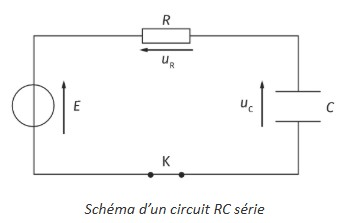
\includegraphics[width=6.5cm]{RC_serie.jpg}\\
{\footnotesize\color{uimmgray} Circuit RC série.}
\end{center}

L'équation $RC\,u_C' + u_C = E$ se normalise en $u_C' + \dfrac{1}{RC}\,u_C = \dfrac{E}{RC}$, de constante de temps $\tau = RC$.

\begin{theoreme}
Avec un condensateur initialement déchargé ($u_C(0) = 0$), la tension est :
\[
u_C(t) = E\left(1 - e^{-t/RC}\right).
\]
Le courant, lui, décroît : $i(t) = \dfrac{E}{R}\,e^{-t/RC}$.
\end{theoreme}

\begin{exemple}
$R = 1\,$k$\Omega$, $C = 100\,\mu$F, $E = 5\,$V : $\tau = 0{,}1\,$s.
\[
u_C(\tau) = 5(1 - e^{-1}) \approx 3{,}16\,\text{V}, \qquad u_C(0{,}3) = 5(1 - e^{-3}) \approx 4{,}75\,\text{V}.
\]
\end{exemple}

\subsection{Établissement du courant (circuit RL)}

\begin{theoreme}
Pour $L\,i' + R\,i = E$ avec $i(0) = 0$, de constante de temps $\tau = \dfrac{L}{R}$ :
\[
i(t) = \frac{E}{R}\left(1 - e^{-\frac{R}{L}t}\right).
\]
Le courant tend vers sa valeur permanente $\dfrac{E}{R}$.
\end{theoreme}

\begin{exemple}
$R = 10\,\Omega$, $L = 0{,}5\,$H, $E = 12\,$V : $\tau = 0{,}05\,$s et $i_\infty = 1{,}2\,$A. Après $5\tau = 0{,}25\,$s, le courant a quasiment atteint $1{,}2\,$A.
\end{exemple}

\subsection{Refroidissement après traitement thermique}

\begin{center}
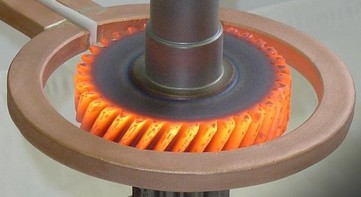
\includegraphics[width=6.5cm]{traitement_thermique.jpg}\\
{\footnotesize\color{uimmgray} Pièce portée à haute température.}
\end{center}

\begin{appliindus}[-- Loi de Newton]
Une pièce sort d'un four à $\theta_0 = 800\,°$C et refroidit dans un atelier à $\theta_a = 20\,°$C, avec $k = 0{,}05\,$min$^{-1}$. L'équation $\theta' + k\theta = k\theta_a$ donne :
\[
\theta(t) = \theta_a + (\theta_0 - \theta_a)\,e^{-kt} = 20 + 780\,e^{-0{,}05\,t}.
\]
\begin{itemize}
  \item $\theta(20) = 20 + 780\,e^{-1} \approx 307\,°$C ;
  \item température de $100\,°$C atteinte pour $t = \dfrac{\ln(780/80)}{0{,}05} \approx 45{,}5\,$min.
\end{itemize}
Ce calcul dimensionne les temps de refroidissement entre deux opérations.
\end{appliindus}

\subsection{Chute avec frottement visqueux}

\begin{center}
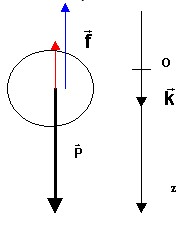
\includegraphics[width=4.2cm]{chute_libre.jpg}\\
{\footnotesize\color{uimmgray} Mobile en chute freinée.}
\end{center}

\begin{appliindus}[-- Vitesse limite]
Un mobile de masse $m$ tombe en subissant un frottement visqueux $-k v$. Le PFD donne $m\,v' = mg - k v$, soit $v' + \dfrac{k}{m}\,v = g$. Avec $v(0) = 0$ :
\[
v(t) = \frac{mg}{k}\left(1 - e^{-\frac{k}{m}t}\right).
\]
La \textbf{vitesse limite} est $v_\infty = \dfrac{mg}{k}$. Pour $m = 0{,}2\,$kg et $k = 0{,}4\,$N$\cdot$s/m : $v_\infty \approx 4{,}91\,$m/s, atteinte en quelques $\tau = m/k = 0{,}5\,$s.
\end{appliindus}

\subsection{Cinétique chimique du premier ordre}

\begin{appliindus}[-- Disparition d'un réactif]
La concentration $[A]$ d'un réactif d'une réaction du premier ordre vérifie $[A]' = -k[A]$, d'où :
\[
[A](t) = [A]_0\,e^{-kt}.
\]
Le \textbf{temps de demi-réaction} $t_{1/2} = \dfrac{\ln 2}{k}$ ne dépend pas de la concentration initiale. Même modèle pour la désintégration radioactive et la dépollution d'un bain.
\end{appliindus}

% ============================================================
% SECTION 8 : EULER
% ============================================================
\newpage
\section{Résolution approchée : la méthode d'Euler}

Quand on ne sait pas résoudre l'équation à la main, on en calcule une solution \textbf{approchée} pas à pas. C'est le principe de la méthode d'Euler.

\begin{methode}[-- Méthode d'Euler pour $y' = g(t, y)$]
On part de la condition initiale $(t_0, y_0)$ et d'un pas $h$. À chaque étape :
\[
t_{n+1} = t_n + h, \qquad y_{n+1} = y_n + h \times g(t_n, y_n).
\]
On approche la courbe par de petits segments de pente $y'$.
\end{methode}

\begin{lstlisting}[style=uimmpython, caption={Méthode d'Euler pour $y' = -2y + 6$, $y(0)=0$}]
h = 0.1          # pas
t, y = 0, 0      # condition initiale
for n in range(5):
    y = y + h * (-2 * y + 6)   # y' = -2y + 6
    t = t + h
    print(round(t, 1), round(y, 4))
\end{lstlisting}

\begin{exemple}[-- Comparaison avec la solution exacte]
Pour $y' + 2y = 6$, $y(0) = 0$, la solution exacte est $y(t) = 3(1 - e^{-2t})$. Avec $h = 0{,}1$ :
\begin{center}
\renewcommand{\arraystretch}{1.3}
\begin{tabular}{|c|c|c|c|c|c|c|}
\hline
\rowcolor{uimmlightblue}
$t$ & $0$ & $0{,}1$ & $0{,}2$ & $0{,}3$ & $0{,}4$ & $0{,}5$ \\
\hline
Euler & $0$ & $0{,}60$ & $1{,}08$ & $1{,}46$ & $1{,}77$ & $2{,}02$ \\
\hline
Exact & $0$ & $0{,}54$ & $0{,}99$ & $1{,}35$ & $1{,}65$ & $1{,}90$ \\
\hline
\end{tabular}
\end{center}
La méthode d'Euler suit la tendance mais accumule une erreur : plus le pas $h$ est petit, plus l'approximation est fine.
\end{exemple}

\begin{remarque}
Un logiciel (tableur, Python, calculatrice) permet aussi de \textbf{représenter la famille des courbes solutions} en faisant varier la constante $C$ ou la condition initiale, ce qui est une capacité attendue du programme.
\end{remarque}

% ============================================================
% SECTION 9 : EXERCICES
% ============================================================
\newpage
\section{Exercices d'application}

\subsection*{Exercice 1 -- Équations homogènes}
Résoudre les équations différentielles suivantes :
\begin{enumerate}[label=\alph*)]
  \item $y' + 5y = 0$ ;
  \item $3y' + 6y = 0$ ;
  \item $y' - 4y = 0$.
\end{enumerate}

\subsection*{Exercice 2 -- Avec second membre}
Donner la solution générale de :
\begin{enumerate}[label=\alph*)]
  \item $y' + 2y = 8$ ;
  \item $y' + y = 3t$ ;
  \item $y' - 2y = e^{3t}$.
\end{enumerate}

\subsection*{Exercice 3 -- Problème de Cauchy}
Résoudre $y' + 4y = 12$ avec $y(0) = 1$, puis préciser la limite de $y$ en $+\infty$.

\subsection*{Exercice 4 -- Circuit RC}
Un circuit RC série a $R = 2\,$k$\Omega$ et $C = 250\,\mu$F. On applique à $t = 0$ une tension $E = 10\,$V sur un condensateur déchargé.
\begin{enumerate}[label=\alph*)]
  \item Écrire l'équation différentielle vérifiée par $u_C(t)$ et donner la constante de temps $\tau$.
  \item Résoudre et donner $u_C(t)$.
  \item Calculer $u_C(\tau)$ et le temps au bout duquel $u_C$ atteint $9\,$V.
\end{enumerate}

\subsection*{Exercice 5 -- Circuit RL}
Une bobine $L = 0{,}2\,$H en série avec $R = 8\,\Omega$ est branchée sur $E = 24\,$V à $t = 0$ ($i(0) = 0$).
\begin{enumerate}[label=\alph*)]
  \item Établir l'équation différentielle vérifiée par $i(t)$.
  \item Donner $i(t)$ et la valeur du courant en régime permanent.
  \item Calculer la constante de temps et le temps de réponse à $5\,\%$.
\end{enumerate}

\subsection*{Exercice 6 -- Refroidissement}
Une pièce métallique à $600\,°$C refroidit dans un local à $25\,°$C. On mesure un coefficient $k = 0{,}03\,$min$^{-1}$.
\begin{enumerate}[label=\alph*)]
  \item Écrire l'équation vérifiée par $\theta(t)$ et la résoudre.
  \item Calculer la température au bout de $30\,$min.
  \item Déterminer le temps nécessaire pour descendre sous $100\,°$C (manipulation possible).
\end{enumerate}

\subsection*{Exercice 7 -- Méthode d'Euler}
On considère $y' = -y + 2$ avec $y(0) = 0$.
\begin{enumerate}[label=\alph*)]
  \item Donner la solution exacte.
  \item Appliquer la méthode d'Euler avec un pas $h = 0{,}2$ pour estimer $y(0{,}2)$, $y(0{,}4)$ et $y(0{,}6)$.
  \item Comparer $y(0{,}6)$ approché à la valeur exacte.
\end{enumerate}

% ============================================================
% FORMULAIRE
% ============================================================
\newpage
\section*{Formulaire -- À retenir}
\addcontentsline{toc}{section}{Formulaire}

\begin{tcolorbox}[colback=uimmlightblue, colframe=uimmblue, title={\textbf{Formulaire des équations différentielles du 1\textsuperscript{er} ordre}}, fonttitle=\large\bfseries\sffamily, coltitle=white, boxrule=1.5pt, arc=5pt]

\textbf{Forme générale :} $a\,y' + b\,y = c(t)$, \; forme normalisée $y' + \alpha y = f(t)$ avec $\alpha = \dfrac{b}{a}$.

\vspace{6pt}
\textbf{Équation homogène :} $y' + \alpha y = 0 \;\Rightarrow\; y_h(t) = C\,e^{-\alpha t}$.

\vspace{6pt}
\textbf{Solution générale :} $y(t) = y_h(t) + y_p(t)$ (transitoire $+$ permanent).

\vspace{4pt}
\renewcommand{\arraystretch}{1.6}
\begin{tabular}{|>{\raggedright\arraybackslash}m{5.2cm}|>{\raggedright\arraybackslash}m{9cm}|}
\hline
\rowcolor{uimmblue!20}
\textbf{Second membre $c(t)$} & \textbf{Forme de la solution particulière $y_p$} \\
\hline
constante $K$ & $y_p = K/b$ \\
\hline
polynôme de degré $n$ & polynôme de degré $n$ (identification) \\
\hline
$P\,e^{\gamma t}$, $\gamma \neq -\alpha$ & $y_p = \lambda\,e^{\gamma t}$ \\
\hline
$P\cos\omega t + Q\sin\omega t$ & $y_p = \lambda\cos\omega t + \mu\sin\omega t$ \\
\hline
\end{tabular}

\vspace{8pt}
\textbf{Condition initiale :} $y(t_0) = y_0$ détermine la constante $C$ (solution unique).

\vspace{6pt}
\textbf{Constante de temps :} $\tau = \dfrac{1}{\alpha}$ ; \; $y(t) = y_\infty + (y_0 - y_\infty)e^{-t/\tau}$ ; \; $63\,\%$ à $\tau$, $99\,\%$ à $5\tau$.

\vspace{6pt}
\textbf{Méthode d'Euler :} $y_{n+1} = y_n + h\,g(t_n, y_n)$ pour $y' = g(t,y)$.

\vspace{4pt}
\textbf{Modèles types :} RC $\to \tau = RC$ ; \; RL $\to \tau = L/R$ ; \; refroidissement $\theta = \theta_a + (\theta_0-\theta_a)e^{-kt}$.
\end{tcolorbox}

\vfill
\begin{center}
\color{uimmgray}\small
\textit{Document réalisé par le Pôle Formation UIMM -- Centre-Val de Loire}\\
\textit{La Fabrique de l'Avenir -- S. JAUBERT}
\end{center}

\end{document}
